\let\negmedspace\undefined
\let\negthickspace\undefined
\documentclass[journal]{IEEEtran}
\usepackage[a5paper, margin=10mm, onecolumn]{geometry}
%\usepackage{lmodern} % Ensure lmodern is loaded for pdflatex
\usepackage{tfrupee} % Include tfrupee package

\setlength{\headheight}{1cm} % Set the height of the header box
\setlength{\headsep}{0mm}     % Set the distance between the header box and the top of the text

\usepackage{gvv-book}
\usepackage{gvv}
\usepackage{cite}
\usepackage{amsmath,amssymb,amsfonts,amsthm}
\usepackage{algorithmic}
\usepackage{graphicx}
\usepackage{textcomp}
\usepackage{xcolor}
\usepackage{txfonts}
\usepackage{listings}
\usepackage{enumitem}
\usepackage{mathtools}
\usepackage{gensymb}
\usepackage{comment}
\usepackage[breaklinks=true]{hyperref}
\usepackage{tkz-euclide} 
\usepackage{listings}
\usepackage{gvv}
\usepackage{tikz}
\def\inputGnumericTable{}                                 
\usepackage[latin1]{inputenc}                                
\usepackage{color}                                            
\usepackage{array}                                            
\usepackage{longtable}                                       
\usepackage{calc}                                             
\usepackage{multirow}                                         
\usepackage{hhline}                                           
\usepackage{ifthen}                                           
\usepackage{lscape}
\begin{document}

\bibliographystyle{IEEEtran}
\vspace{3cm}

\title{Gate Questions}
\author{EE24BTECH11013-DASARI MANIKANTA
}
 \maketitle
% \newpage
% \bigskip
{\let\newpage\relax\maketitle}

\renewcommand{\thefigure}{\theenumi}
\renewcommand{\thetable}{\theenumi}
\setlength{\intextsep}{10pt} % Space between text and floats


\numberwithin{equation}{enumi}
\numberwithin{figure}{enumi}
\renewcommand{\thetable}{\theenumi}
\begin{enumerate}
\item  The energy levels of a particle of mass $m$ in a potential of the form

$
V(x) =
\begin{cases} 
\infty, & x \leq 0 \\
\frac{1}{2} m \omega^2 x^2, & x > 0
\end{cases} $

are given, in terms of quantum number $n = 0, 1, 2, 3, \dots$, by

\begin{enumerate}
\item $ \left(n + \frac{1}{2}\right)\hbar\omega \quad $
\item $ \left(2n + \frac{1}{2}\right)\hbar\omega \quad $
\item $ \left(2n + \frac{3}{2}\right)\hbar\omega \quad $
\item $ \left(n + \frac{3}{2}\right)\hbar\omega $
\end{enumerate}

\item The electromagnetic field due to a point change must be described by Lienard-Weichert potentials when 
\begin{enumerate}
    \item  the point charge is highly accelerated,
\item the electric and magnetic fields are not perpendicular.
\item the point charge is moving with velocity close to that of light.
\item the calculation is done for the radiation zone, i.e far away from the charge.
\end{enumerate}
\item The starngeness quantum numbers is conserved in 
\begin{enumerate}
\item strong,weak and electromagnetic interactions .
    \item weak and electromagnetic interactions only.
    \item strong and weak interactions only.
    \item strong and electromagnetic interactions only.
\end{enumerate}
\item The eigenvalues and eigenvectors of the matrix 
\[
\begin{bmatrix}
5 & 4 \\
1 & 2
\end{bmatrix}
\]
are

\begin{enumerate}
\item $6, 1$ \text{ and } 
$\begin{bmatrix} $4$ \\ $1$ \end{bmatrix}$ 
$\begin{bmatrix} $1$ \\ $-1$ \end{bmatrix}$
\item $2, 5$ \text{ and } 
$\begin{bmatrix} $4$ \\ $1$ \end{bmatrix}$ 
$\begin{bmatrix} $1$ \\ $-1$ \end{bmatrix}$
\item  $6, 1$ \text{ and } 
$\begin{bmatrix} $1$ \\ $4$ \end{bmatrix}$ 
$\begin{bmatrix} $1$ \\ $-1$ \end{bmatrix}$
\item $2, 5$ \text{ and } 
$\begin{bmatrix} $1$ \\ $4$ \end{bmatrix}$ 
$\begin{bmatrix} $1$ \\ $-1$ \end{bmatrix}$
\end{enumerate}
\newpage
\item A vector field is defined everywhere as $\vec{F} = -\frac{y^2}{L} \hat{i} + z \hat{k}$. The net flux of $\vec{F}$ associated with a cube of side $L$, with one vertex at the origin and sides along the positive $X$, $Y$, and $Z$ axes, is

\begin{enumerate}
\item $2L^3$ \quad
\item $4L^3$ \quad
\item $8L^3$ \quad
\item $10L^3$
\end{enumerate}


\item If $\vec{r} = x \hat{i} + y \hat{j}$, then


\begin{enumerate}

\item $\nabla \cdot \vec{r} = 0 \text{ and } \nabla |\vec{r}| = \frac{\vec{r}}{r}$

\item $\nabla \cdot \vec{r} = 2 \text{ and } \nabla |\vec{r}| = \hat{r}$

\item $\nabla \cdot \vec{r} = 2 \text{ and } \nabla |\vec{r}| = \frac{\vec{r}}{r}$

\item $\nabla \cdot \vec{r} = 3 \text{ and } \nabla |\vec{r}| = \frac{\vec{r}}{r}$
\end{enumerate}
\item Consider a vector $\vec{p} = 2\hat{i} + 3\hat{j} + 2\hat{k}$ in the coordinate system $(\hat{i}, \hat{j}, \hat{k})$. The axes are rotated anti-clockwise about the $Y$ axis by an angle of $60^\circ$. The vector $\vec{p}$ in the rotated coordinate system $(\hat{i'}, \hat{j'}, \hat{k'})$ is

\begin{enumerate}
\item $(1-\sqrt{3})\hat{i'} + 3\hat{j'} + (1+\sqrt{3})\hat{k'}$

\item $(1+\sqrt{3})\hat{i'} + 3\hat{j'} + (1-\sqrt{3})\hat{k'}$

\item $(1-\sqrt{3})\hat{i'} + (3+\sqrt{3})\hat{j'} + 2\hat{k'}$


\item $(1-\sqrt{3})\hat{i'} + (3-\sqrt{3})\hat{j'} + 2\hat{k'}$
\end{enumerate}
\item The contour integral \( \oint \frac{dz}{z^4 + a^4} \)is to be evaluated on a circle of radius $2a$ centered at the origin. It will have contributions only from the points
\begin{enumerate}
\item $\ \frac{1+i}{\sqrt{2}}a \ \text{and} \ \frac{1-i}{\sqrt{2}}a$

\item  \ $ia$ \ \text{and} \ $-ia$
\item $ \ $ia$, \ $-ia$, \ \frac{-i}{\sqrt{2}}a \ \text{and} \ \frac{1-i}{\sqrt{2}}a$
\item $ \ \frac{1+i}{\sqrt{2}}a, \ \frac{1-i}{\sqrt{2}}a, \ \frac{-i}{\sqrt{2}}a \ \text{and} \ \frac{1-i}{\sqrt{2}}a$
\end{enumerate}
\item Inverse Laplace transform of \( \frac{s+1}{s^2 - 4}\) is
\begin{enumerate}
\item $\ \cos 2x + \frac{1}{2}\sin 2x$
\item $ \ \cos x + \frac{1}{2}\sin x$

\item $\ \cosh x + \frac{1}{2}\sinh x$
\item $\ \cosh 2x + \frac{1}{2}\sinh 2x$
\end{enumerate}
\item The points, where the series solution of the Legendre differential equation
\[
(1 - x^2)\frac{d^2 y}{dx^2} - 2x\frac{dy}{dx} + \frac{3}{2}\left(\frac{3}{2}+1\right)y = 0 
\]
will diverge, are located at
\begin{enumerate}
\item $ \ 0 \ \text{and} \ 1$
\item $ \ 0 \ \text{and} \ -1$
\item $ \ -1 \ \text{and} \ 1$
\item $ \ \frac{3}{2} \ \text{and} \ \frac{5}{2} $
\end{enumerate}
\newpage
\item Solution of the differential equation \( x \frac{dy}{dx} + y = x^4 \), with the boundary condition that \( y = 1 \) at \( x = 1 \), is
\begin{enumerate}
\item $ \ y = 5x^4 - 4$
\item $\ y = \frac{x^4}{5} + \frac{4x}{5} $
\item $ \ y = \frac{4x^4}{5} + \frac{1}{5x} $
\item $\ y = \frac{x^4}{5} + \frac{4}{5x} $
\end{enumerate} 
\item Match the following \\ \[
\begin{array}{cl}
\text{P.} & \text{rest mass} \\
\text{Q.} & \text{charge} \\
\text{R.} & \text{four-momentum} \\
\text{S.} & \text{electromagnetic field} \\
\end{array}
\quad
\begin{array}{cl}
1. & \text{timelike vector} \\
2. & \text{Lorentz invariant} \\
3. & \text{tensor of rank 2} \\
4. & \text{conserved and Lorentz invariant} \\
\end{array}
\]
\begin{enumerate}
    \item $P-2,Q-4,R-3,S-1$
    \item $P-4,Q-2,R-1,S-3$
    \item $P-2,Q-4,R-1,S-3$
    \item $P-4,Q-2,R-3,S-1$
    \end{enumerate}

\item The moment of inertia of a uniform sphere of radius \( r \) about an axis passing through its center is given by
\[
\frac{2}{5} \left( \frac{4\pi}{3} r^3 \rho \right)
\]
A rigid sphere of uniform mass density \( \rho \) and radius \( R \) has two smaller spheres of radius \( R/2 \) hollowed out of it, as shown in the figure. The moment of inertia of the resulting body about the Y axis is:
\begin{center}
\begin{tikzpicture}
    % Draw the large circle
    \draw (0,0) circle (2cm);
    
    % Draw the two smaller circles inside the large one
    \draw (-1,0) circle (1cm);
    \draw (1,0) circle (1cm);
    
    % Draw the coordinate axes
    \draw[->] (0,-2.5) -- (0,2.5) node[above] {$Y$};
    \draw[->] (-2.5,0) -- (2.5,0) node[right] {$X$};
\end{tikzpicture}
\end{center}
\begin{enumerate}
\item $ \ \frac{\pi \rho R^5}{4}
\quad $
\item $ \ \frac{5\pi \rho R^5}{12}
\quad $
\item $ \ \frac{7\pi \rho R^5}{12}
\quad $
\item $ \ \frac{3\pi \rho R^5}{4}
$
\end{enumerate}
\newpage
\item The Lagrangian of a particle of mass \( m \) is

$L = \frac{m}{2} \left[ \left( \frac{dx}{dt} \right)^2 + \left( \frac{dy}{dt} \right)^2 + \left( \frac{dz}{dt} \right)^2 \right] - \frac{V}{2} \left( x^2 + y^2 \right) + W \sin \omega t $

where \( V \), \( W \), and \( \omega \) are constants. The conserved quantities are:
\begin{enumerate}
\item $\ \text{energy and z-component of linear momentum only.}$
\item $ \ \text{energy and z-component of angular momentum only.} $
\item $\ \text{z-components of both linear and angular momenta only.} $
\item $\ \text{energy and z-components of both linear and angular momenta.}$
\end{enumerate} 
\item Three particles of mass \( m \), each situated at \( x_1(t) \), \( x_2(t) \), and \( x_3(t) \) respectively, are connected by two springs of spring constant \( k \) and un-stretched length \( \ell \). The system is free to oscillate only in one dimension along the straight line joining all three particles. The Lagrangian of the system is:
\begin{enumerate}
\item $ \ L = \frac{m}{2} \left[ \left( \frac{dx_1}{dt} \right)^2 + \left( \frac{dx_2}{dt} \right)^2 + \left( \frac{dx_3}{dt} \right)^2 \right] - \frac{k}{2} (x_1 - x_2 - \ell)^2 - \frac{k}{2} (x_3 - x_2 - \ell)^2$
\item $ \ L = \frac{m}{2} \left[ \left( \frac{dx_1}{dt} \right)^2 + \left( \frac{dx_2}{dt} \right)^2 + \left( \frac{dx_3}{dt} \right)^2 \right] - \frac{k}{2} (x_1 - x_3 - \ell)^2 - \frac{k}{2} (x_3 - x_2 - \ell)^2$
\item $ \ L = \frac{m}{2} \left[ \left( \frac{dx_1}{dt} \right)^2 + \left( \frac{dx_2}{dt} \right)^2 + \left( \frac{dx_3}{dt} \right)^2 \right] - \frac{k}{2} (x_1 - x_2 + \ell)^2 - \frac{k}{2} (x_3 - x_2 + \ell)^2$
\item $ \ L = \frac{m}{2} \left[ \left( \frac{dx_1}{dt} \right)^2 + \left( \frac{dx_2}{dt} \right)^2 + \left( \frac{dx_3}{dt} \right)^2 \right] - \frac{k}{2} (x_1 - x_2 - \ell)^2 - \frac{k}{2} (x_3 - x_2 + \ell)^2$
\end{enumerate}
\item The Hamiltonian of a particle is \( H = \frac{p^2}{2m} + pq \), where  $q$ is the generalized coordinate and  $p$  is the corresponding canonical momentum. The Lagrangian is

\begin{enumerate}
\item $ \quad \frac{m}{2} \left( \frac{dq}{dt} + q \right)^2 $
\item $ \quad \frac{m}{2} \left( \frac{dq}{dt} - q \right)^2 $
\item $ \quad \frac{m}{2} \left( \frac{dq}{dt} \right)^2 + q \frac{dq}{dt} - q^2 $
\item $ \quad \frac{m}{2} \left( \frac{dq}{dt} \right)^2 - q \frac{dq}{dt} + q^2 $
\end{enumerate}
\item A toroidal coil has  $N$  closely-wound turns. Assume the current through the coil to be $I$ and the toroid is filled with a magnetic material of relative permittivity $ \mu_r$ . The magnitude of magnetic induction $\vec{B} $ inside the toroid, at a radial distance $r$  from the axis, is given by

\begin{enumerate}
\item $ \quad \mu_r \mu_0 NIr $
\item $\quad \frac{\mu_r \mu_0 NI}{r} $
\item $ \quad \frac{\mu_r \mu_0 NI}{2 \pi r} $
\item $\quad \frac{2 \pi \mu_r \mu_0 NIr}{r} $
\end{enumerate}




\end{enumerate}
\end{document}
